\section{State of the Art}\label{soa}
Early civil aviation primarily relied on primary and secondary radars, which had limitations such as limited detection range, insufficient information accuracy, and delayed updates. These shortcomings not only increased the navigation difficulty for long-distance flights but also posed safety risks\cite{icao_1993}.
To address these challenges, the aviation industry has gradually developed the ADS-B system through decades of exploration. Relying on the Global Navigation Satellite System (GNSS) and on-board sensors, ADS-B integrates information such as barometric altitude, inertial navigation, and airspeed measurements to generate flight status parameters. It then periodically broadcasts key data like identification codes, position, altitude, speed, and flight intentions via on-board equipment \cite{olive2024filtering}.

The development of ADS-B can be traced back to the 1970s. In 2003, the 11th Air Navigation Conference of the International Civil Aviation Organization (ICAO) \cite{icao_2003} formally recognized ADS-B as a key surveillance tool for future air traffic management and promoted its standardization and application.
After 2010, ADS-B entered the phase of large-scale global application. Countries have successively introduced regulations to promote its widespread use in aviation operations. Meanwhile, the application of space-based ADS-B \cite{melero2024satera} has enabled real-time, high-precision surveillance of approximately (70\%) of the world's airspace. Open platforms represented by the OpenSky Network \cite{schafer2014bringing} have also provided large-scale ADS-B data resources for academic research.

\subsection{ADS-B Data current usages}

This section presents an overview of the current use of ADS-B data in the research domain, identifying and organizing clusters of algorithms and application areas. In this study, the collected literature is categorized into eight major domains, spanning from trajectory modeling and operational management to environmental sustainability and cybersecurity. These analyses provide a structured overview of the evolving research landscape surrounding ADS-B applications in aviation.

\subsubsection{Paper Selection}

To ensure both representativeness and research quality, we focused on journals and conferences with high academic impact in the fields of air traffic management (ATM) and digital aviation. The primary sources include the \textit{Digital Avionics Systems Conference (DASC)}, \textit{SESAR Joint Undertaking Annual Conference}, \textit{Air Traffic Management Seminar (ATM Seminar)}, \textit{International Conference on Research in Air Transportation (ICRAT)}, \textit{Transportation Research Part C: Emerging Technologies}, \textit{IEEE Transactions on Intelligent Transportation Systems}, and the \textit{Journal of Air Transport Management (JATM)}. Literature retrieval was mainly conducted through academic databases such as IEEE Xplore, ScienceDirect, and Elsevier Scopus, as well as publicly available proceedings from the aforementioned conferences.

Considering that large-scale implementation and operational use of ADS-B systems began worldwide around 2012, this year was set as the starting point for the large-scale research phase of ADS-B data. Therefore, this study selected English-language publications issued between 2012 and December 2024 as the objects of analysis. We manually collected research that explicitly utilized real ADS-B flight data from the selected journals and conferences, excluding studies that relied solely on simulated or synthetic datasets.
The detailed screening process was as follows:

\begin{itemize}
	\item \textbf{Initial Screening:} Titles and abstracts were reviewed to confirm the study’s relevance to the aviation domain, such as airspace optimization, trajectory prediction, or conflict detection and avoidance (DAA).
	\item \textbf{Keyword Filtering:} Only papers containing the term ``ADS-B'' in the title, abstract, or keywords were retained.
	\item \textbf{Data Authenticity Criterion:} Studies were required to clearly indicate the use of real ADS-B datasets. Papers using only simulated or artificially generated trajectories were excluded.
	\item \textbf{Duplication and Accessibility Review:} Duplicate publications and inaccessible preprints were removed to ensure the reproducibility and verifiability of the results.
\end{itemize}

After multiple rounds of screening and manual verification, a total of 145 papers were collected, covering representative applications of ADS-B data across diverse research domains. The distribution of the selected studies by source is illustrated in Figure ~\ref{fig:placeholder}.


\begin{figure}
	\centering
	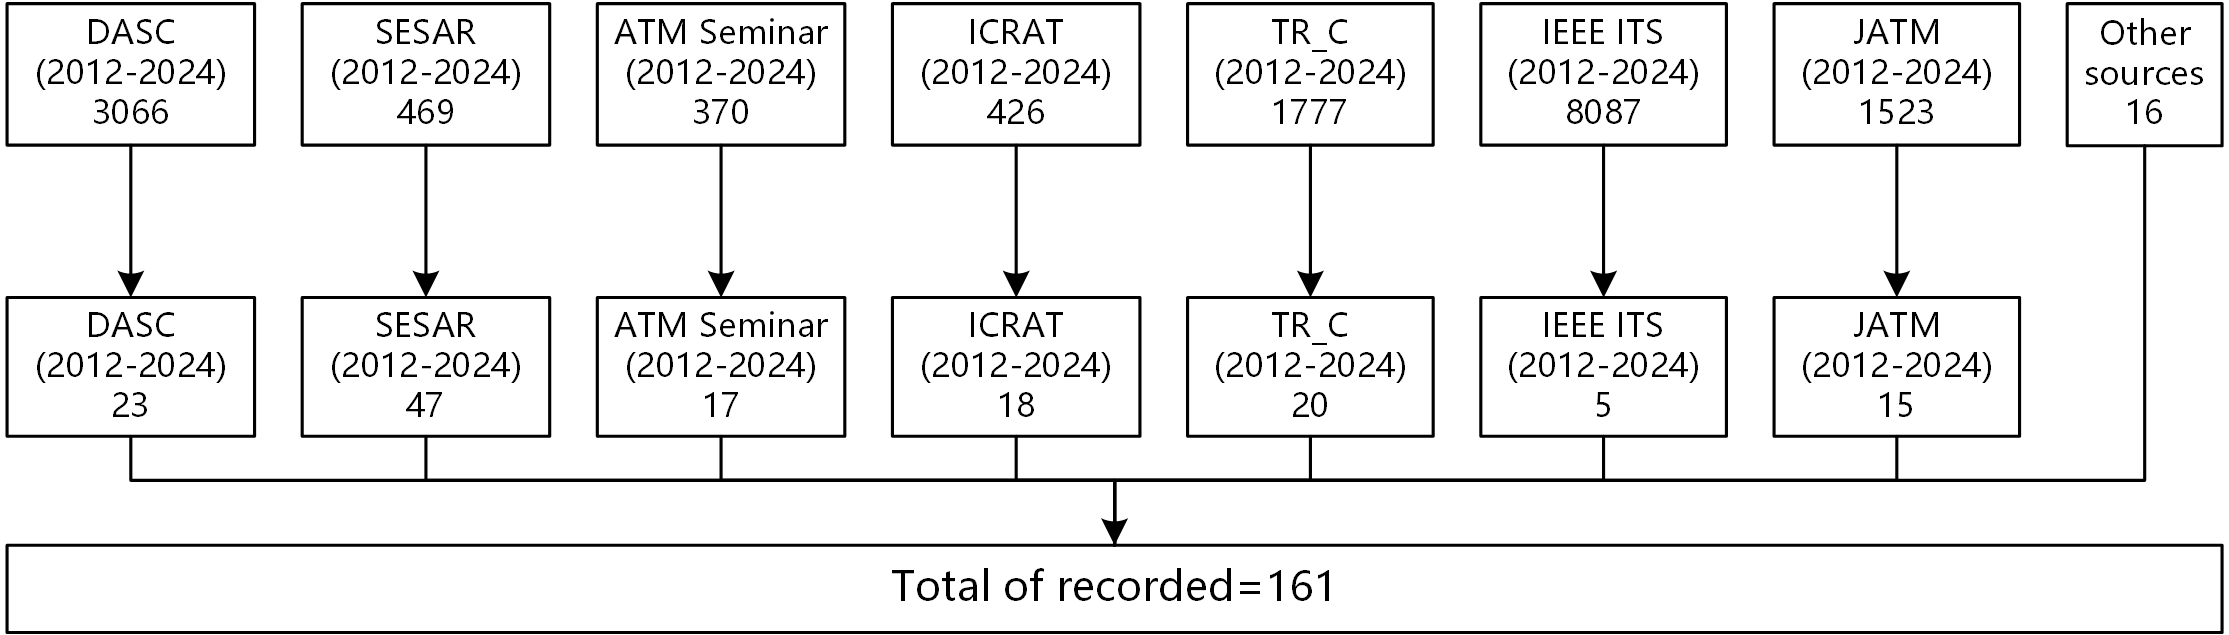
\includegraphics[width=1\linewidth]{paper_selection.png}
	\caption{Paper collection flow of the review made on Digital Avionics Systems Conference (DASC), SESAR Joint Undertaking Annual Conference (SESAR), Air Traffic Management Research and Development Seminar (ATM seminar), International Conference on Research in Air Transportation (ICRAT), Transportation Research Part C: Emerging Technologies (TR\_C), Journal of Air Transport Management (JATM), and IEEE Transactions on Intelligent Transportation Systems (IEEE Trans. on ITS).}
	\label{fig:placeholder}
\end{figure}


\subsubsection{Paper Clustering and Categorization}

The screened publications provided a solid data foundation for the categorization and trend analysis of ADS-B applications in this study. To systematically organize the characteristics and focal points of different research directions, we employed a mixed quantitative–qualitative approach for feature extraction and clustering of the collected literature.

Using Excel spreadsheets and reference management tools, the following key features were extracted from each selected conference and journal:
Publication year; Source conference or journal; Paper title and author keywords; Application scenario; Research focus or analytical perspective; Methods and algorithmic approaches (e.g., machine learning, optimization models, statistical analysis, simulation frameworks); Description of the ADS-B dataset used (e.g., public data repositories, airport-specific data, or crowdsourced datasets).

In the preliminary organization stage, the literature was grouped into four broad directions: trajectory prediction, air traffic management, aircraft performance estimation, and environmental sustainability. However, a subsequent semantic and thematic analysis revealed substantial overlaps and hierarchical relationships among these themes. Therefore, this study reclassified the literature through a combined thematic synthesis approach, considering each study’s research objectives, data utilization patterns, and the functional role of ADS-B. Finally, ADS-B–related studies were categorized into eight major domains:
Trajectory Modeling and Prediction, Operational Optimization and Management, Operational Safety and Surveillance, Aircraft Performance and Efficiency, Data Engineering and Enhancement, Environment and Sustainability, Security and Cybersecurity, Methodology, Simulation, and Policy. This classification framework establishes the structural foundation for the domain-specific analyses presented in the following sections. The classification results, derived from thematic induction and semantic grouping, are summarized in Table \ref{tb:8categories}, illustrating the representative applications and algorithms across the eight research domains.

\begin{table}[htbp]
	\centering
	\caption{Summary of ADS-B Application Categories, Main Methods, and Data Roles}
	\label{tb: 8categories}
	\renewcommand{\arraystretch}{1.15} % 行距
	\setlength{\tabcolsep}{5pt} % 列间距
	\begin{tabular}{p{3.5cm} p{4.5cm} p{3.5cm}}
		\hline
		\textbf{Category} & \textbf{Main Methods} & \textbf{Role of ADS-B Data} \\
		\hline
		\textbf{Trajectory Modeling and Prediction} &
		\makecell[l]{Clustering (DBSCAN, K-means);\\
			LSTM/Transformer prediction;\\
			AE feature extraction; DTW; PCA;\\
			Hybrid physical–data models.} &
		\textbf{Core data source} \\
		\hline
		
		\textbf{Operational Optimization and Management} &
		\makecell[l]{
			MILP; Simulated annealing;\\
			Heuristic algorithms;\\
			KPI-based performance metrics;\\
			Historical traffic analysis.
		} &
		\textbf{Real-time/historical traffic input} \\
		\hline
		
		\textbf{Operational Safety and Surveillance} &
		\makecell[l]{
			DAA geometric models;\\
			Anomaly detection (thresholds,\\ clustering, autoencoder, GMM);\\
			Monte Carlo risk evaluation.
		} &
		\textbf{Flight monitoring and safety baseline} \\
		\hline
		
		\textbf{Aircraft Performance and Efficiency} &
		\makecell[l]{
			Dynamic equation inversion;\\
			Maximum likelihood estimation;\\
			Bayesian inference; Particle filtering;\\
			Regression and neural networks.
		} &
		\textbf{Model calibration data source} \\
		\hline
		
		\textbf{Data Engineering and Enhancement} &
		\makecell[l]{
			Kalman filtering; Map-matching;\\
			Multisource fusion; Data indexing;\\
			Generative models (TimeGAN).
		} &
		\textbf{Primary processing object} \\
		\hline
		
		\textbf{Environment and Sustainability} &
		\makecell[l]{
			Trajectory-based emission estimation;\\
			Remote sensing data fusion;\\
			Optimal control route planning.
		} &
		\textbf{Environmental assessment input} \\
		\hline
		
		\textbf{Security and Cybersecurity} &
		\makecell[l]{
			Intrusion detection (ML classifiers);\\
			Protocol vulnerability testing;\\
			SDR signal analysis.
		} &
		\textbf{Research target} \\
		\hline
		
		\textbf{Methodology, Simulation, and Policy} &
		\makecell[l]{
			Open-source simulation platform\\ development; 
			Data standardization;\\
			Policy and privacy analysis.
		} &
		\textbf{Research infrastructure and policy object} \\
		\hline
	\end{tabular}
	\label{tb:8categories}
\end{table}

\textbf{Trajectory Modeling and Prediction.} 
This domain focuses on modeling and predicting aircraft trajectories based on historical and real-time data. Core tasks include 4D prediction, ETA estimation, trajectory clustering, and uncertainty quantification. As a core data source, ADS-B provides continuous, high-precision position, velocity, and altitude data that determine model accuracy. Gui et al. \cite{xuhao2021trajectory} proposed a semantic trajectory representation for arrival flight clustering to support airspace design, flow management, and ETA estimation; Wang et al. \cite{wang2017short} applied PCA-based dimensionality reduction and Density-Based Spatial Clustering of Applications with Noise (DBSCAN) clustering for preprocessing, followed by a Multi-Cell Neural Network for short-term trajectory prediction in terminal maneuvering areas; and Wang et al. \cite{wang2018hybrid} integrated clustering-based preprocessing with hybrid MCNN models to improve ETA prediction accuracy.

\textbf{Operational Optimization and Management.} 
This domain focuses on improving the overall efficiency of airspace and airport operations, encompassing air traffic flow management, surface operations (taxiing and sequencing), terminal maneuvering area coordination, and airspace structure optimization. ADS-B data play a central role by providing continuous and fine-grained historical and real-time traffic information, serving as a reliable input for optimization models and decision-support systems. It enables accurate operational performance evaluation and data-driven strategy optimization. Research in this area often applies Linear Programming, Simulated Annealing, and heuristic algorithms to address sequencing, scheduling, and routing problems. Other studies employ queuing models and Key Performance Indicators (KPIs) for operational assessment or mine historical ADS-B data to identify bottlenecks such as taxiway congestion and sector capacity limits. Basora et al. \cite{basora2018occupancy} combined DBSCAN clustering with Random Forest regression for sector occupancy prediction, and Delahaye et al. \cite{delahaye2022air} used hierarchical clustering with Transformer models for flow pattern detection and capacity management.

\textbf{Operational Safety and Surveillance.} 
This research domain aims to enhance aviation safety and situational awareness through data-driven analysis. It covers conflict detection and resolution (DAA / ACAS), abnormal event detection (e.g., go-arounds, unstable approaches), assessment of collision risk and airspace complexity, and performance evaluation of surveillance systems. As an independent surveillance source, ADS-B data provide continuous and high-precision trajectory and state information, enabling real-time monitoring of aircraft behavior, detection of potential conflicts and anomalies, and quantitative assessment of operational safety.
Bonifazi et al. \cite{bonifazi2021modeling} identified unstable approaches and go-arounds using ADS-B data, employing rule-based methods and Gaussian Mixture Models for anomaly detection and integrating runway and weather information for improved accuracy. Rorie et al. \cite{rorie2024detect} conducted the first real-world evaluation of the ACAS Xr airborne collision avoidance system. Zhang et al. \cite{zhang2024study} investigated conflict-free routing strategies and compared multiple optimization algorithms, while Bao et al. \cite{bao2024exploring} proposed a multi-airport terminal area risk prediction framework to assess inter-airport conflict probabilities. 

\textbf{Aircraft Performance and Efficiency.} 
This research area focuses on deriving aircraft performance parameters from flight data to calibrate or complement existing models such as BADA, and to evaluate energy efficiency across aircraft types and flight phases. Key parameters include aircraft mass, drag polar, thrust settings, fuel consumption, and speed profiles.
In this context, ADS-B data provide essential flight state information, such as ground speed, vertical rate, and heading—enabling large-scale, fleet-level performance analysis even in the absence of detailed design data. This supports more accurate and data-driven model calibration and validation.
Sun et al. \cite{sun2018aircraft} developed a probabilistic framework to estimate aerodynamic parameters from operational data; Schultz et al. \cite{schultz2022data} integrated FDR and ADS-B data to model fuel consumption and operational efficiency using machine learning methods; and Alligier et al. \cite{alligier2020predictive} predicted aircraft mass and speed intent during climb to enhance physics-based trajectory prediction.

\textbf{Data Engineering and Enhancement.} 
This category focuses on improving the quality and usability of raw ADS-B data, which form the foundation for subsequent analytical and modeling applications. Key tasks include anomaly detection, missing-value imputation, multi-source data fusion, data compression and indexing, and synthetic data generation. In this domain, ADS-B data themselves are the core subject of engineering—aimed at producing cleaner, more complete, and more interoperable datasets that support trajectory prediction, operational analysis, and safety evaluation.
Tabassum et al. \cite{tabassum2017ads} conducted long-term statistical analysis to identify anomalies and assess the impact of systematic errors on trajectory accuracy. Wandelt et al. \cite{wandelt2018ads} introduced an efficient compression and indexing framework to enable scalable querying and analytics of large-scale ADS-B records. Spinielli et al. \cite{spinielli2017initial} developed a reproducible reference trajectory dataset by integrating multiple surveillance sources for performance assessment under the EUROCONTROL PRU initiative.

\textbf{Environment and Sustainability.}
This research area focuses on quantifying the environmental impact of aviation operations and exploring sustainable optimization strategies, including greenhouse gas and pollutant emission assessment, contrail formation detection and avoidance, and noise evaluation. Owing to its wide coverage and high temporal resolution, ADS-B data serve as a crucial source for environmental modeling and validation. For instance, Roosenbrand et al. \cite{roosenbrand2023contrail} proposed a method to estimate contrail altitudes using shadows in Landsat satellite imagery, with ADS-B data employed as ground truth for validation. Sun et al. \cite{sun2023evaluating} integrated satellite-based and ground-based ADS-B data with wind field information to improve emission estimation and compared actual flight trajectories with optimal routes to quantify excess emissions.

\textbf{Security and Cybersecurity.}
This domain focuses on identifying and mitigating cybersecurity threats targeting the ADS-B system itself, such as False Data Injection Attacks (FDIA), signal spoofing, and message tampering, to ensure the integrity and reliability of surveillance information. In this field, the ADS-B protocol, signal, and data link are the direct subjects of vulnerability analysis and protection technology research. For example, Cretin et al.\cite{cretin2018increasing} proposed a Domain-Specific Language-based testing framework to evaluate the resilience of Air Traffic Control systems against FDIA, while Khan et al. \cite{khan2021intrusion} employed machine learning techniques for ADS-B intrusion detection.

\textbf{Methodology, Simulation, and Policy.}
This category provides foundational tools, frameworks, and policy support for aviation research. It includes the development of open-source simulation platforms, advocacy of reproducible research practices, establishment of data standards, and discussion of regulatory and privacy issues related to ADS-B deployment. In this context, ADS-B serves both as input data for constructing realistic scenarios in simulation environments and as a focal topic in advancing data-sharing policies, privacy protection, and industry standards. Mehlitz et al. \cite{mehlitz2019analyzing} proposed the RACE framework for comprehensive airspace data analysis, while Bolic et al. ~\cite{bolic2024roadmap} systematically elaborated on the European ATM Open Science Alliance and its Open Performance Data Initiative (OPDI), which aim to foster transparency and open research in the ATM domain.

%To provide a clearer overview of the application fields of ADS-B data, we conducted a quantitative analysis of field attribution for the 145 valid papers, based on the eight aforementioned classification categories. The results are presented in Figure \ref{fig:paperpiechart2}. It should be noted that some papers cover multiple fields (e.g., Data Engineering + Aircraft Performance Calculation) and are assigned to multiple application fields in accordance with the rule of "counting each involved field separately". Consequently, the total number of papers counted in the pie chart is greater than the actually counted 145 valid samples.

%From the overall distribution, papers related to Operational Optimization and Management represent the most prominent field in ADS-B data research, accounting for 30.6\%. This is followed by Operational Safety and Surveillance (23.6\%) and Trajectory Modeling and Prediction (18.5\%). These three fields collectively account for over 70\% of the total, forming the mainstream directions of ADS-B data applications. This reflects a high alignment between ADS-B data-related research and the core application scenarios of ADS-B: Operational Optimization and Management directly addresses the efficiency needs of ATM systems, such as "improving airspace utilization and reducing flight delays"; meanwhile, Operational Safety and Surveillance, as well as Trajectory Modeling and Prediction, leverage the "real-time positioning and dynamic tracking" capabilities of ADS-B to serve the safety requirements of "flight conflict early warning and rapid identification of abnormal states".
%
%In contrast, the proportions of papers in the fields of Security and Cybersecurity (2.5\%), Environment and Sustainability (5.1\%), and Methodology, Simulation and Policy (5.1\%) are relatively low, collectively accounting for less than 15\%. These fields represent the directions with relatively smaller proportions in current ADS-B data application research.
To illustrate the application domains of ADS-B data, a quantitative analysis was conducted on 145 valid papers according to the eight classification categories, as shown in Figure \ref{fig:paperpiechart2}. Since some studies involve multiple domains (e.g., Data Engineering and Aircraft Performance Calculation), they were counted in each relevant category; thus, the total number in the chart exceeds 145.

Overall, Operational Optimization and Management dominates ADS-B research (30.6\%), followed by Operational Safety and Surveillance (23.6\%) and Trajectory Modeling and Prediction (18.5\%). Together, these account for over 70\% of all studies, reflecting strong alignment with ADS-B’s core functions—enhancing operational efficiency and supporting real-time safety monitoring. In contrast, Security and Cybersecurity (2.5\%), Environment and Sustainability (5.1\%), and Methodology, Simulation, and Policy (5.1\%) remain less represented, indicating emerging but underexplored areas.


\begin{figure}[htbp]
	\centering
	\begin{floatrow}
		% --- 左图 ---
		\ffigbox
		[% 指定 float box 的宽度(与图宽相同)
		0.6\textwidth
		]
		{% 图片内容
			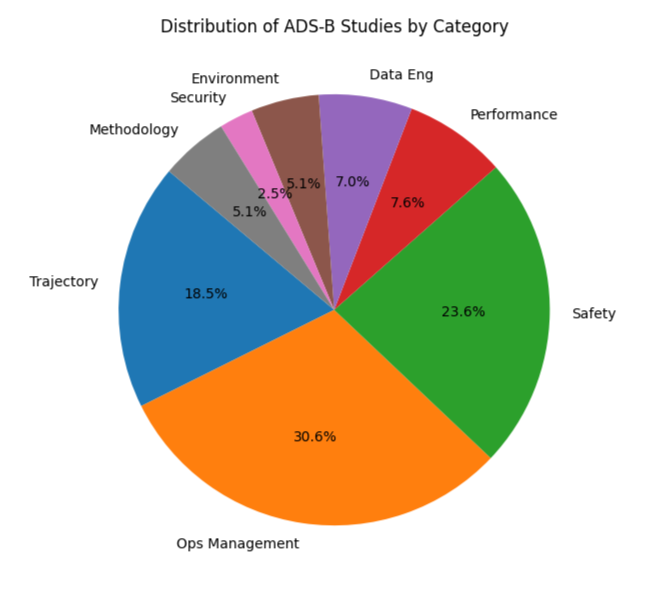
\includegraphics[width=\linewidth, height=5cm, keepaspectratio]{paper_piechart2}
		}
		{% 标题和标签
			\captionsetup{width=\linewidth} % 让标题宽度匹配图片宽度
			\caption{Pie Chart of ADS-B Research Domain Distribution: "Trajectory" for Trajectory Modeling and Prediction; "Ops Management" for Operational Optimization and Management; "Safety" for Operational Safety and Surveillance; "Performance" for Aircraft Performance and Efficiency; "Data Eng" for Data Engineering and Enhancement; "Environment" for Environment and Sustainability; "Security" for Security and Cybersecurity; "Methodology" for Methodology, Simulation, and Policy.}
			\label{fig:paperpiechart2}
		}
		
		\hfill % 控制两图间距
		
		% --- 右图 ---
		\ffigbox
		[0.3\textwidth]
		{% 图片内容
			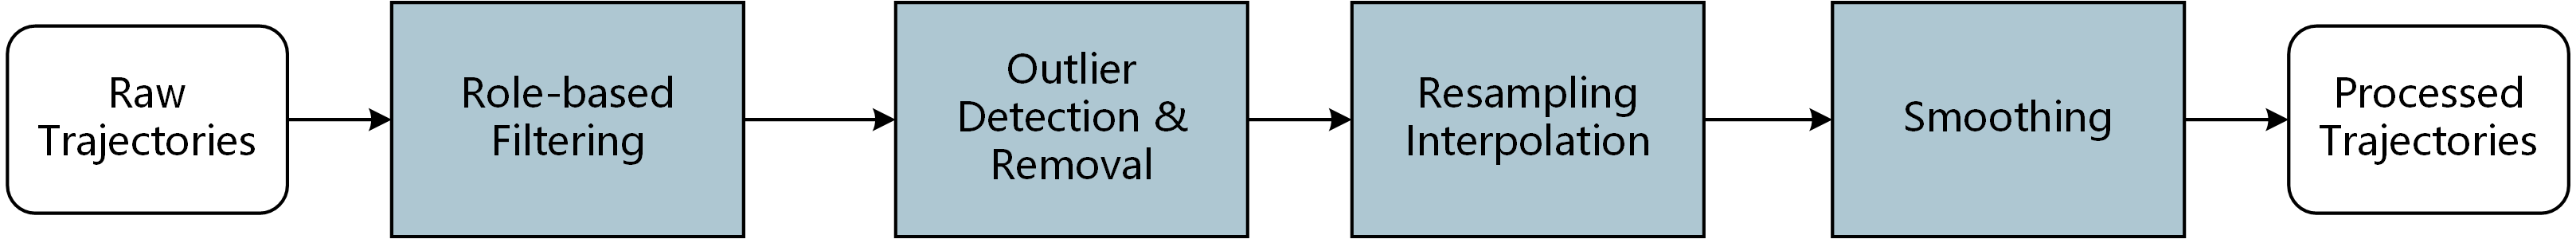
\includegraphics[width=\linewidth, height=5cm, keepaspectratio]{pipeline}
		}
		{% 标题和标签
			\captionsetup{width=\linewidth} % 同理,caption 宽度与图相同
			\caption{Systematic Cleaning Pipeline of ADS-B Trajectories (Raw to Processed) Based on Literature Survey and Taxonomic Summary.}
			\label{fig:Pipeline}
		}
	\end{floatrow}
\end{figure}
